\chapter{Security Policy}
\label{chapter:security_policy}
% \section*{21 - settembre}

\section{Definining Security Policy}
A \textbf{Security Policy} is a set of rules that an organization adopts both to minimize cyber risk and to define the goals of security;
it must:
\begin{itemize}
    \item Define goals of security : assets and resources to protect assets
    \item Define the correct behaviour of all users
    \item Forbid dangerous behaviours and components
    \item Imply the definition of: 
    \begin{itemize}
        \item \textit{System Architecture}, along with a \textit{catalogue} of components and applications, and the \textit{legal use} of resources
        \item \textit{users} and \textit{admins}
        \item Who has to verify that the policy is applied
        \item What happens if the policy is violated
    \end{itemize}
    \item Avoid violating the legislation that concerns ICT systems
\end{itemize}

\section{Terminology}
\subsection{Subject and Object}
\begin{itemize}
    \item \textbf{Subject}: entity which can invoke an operation on an object
    \note{aka \textit{Principal}}
    e.g. User, application, program, process, ... 
    \item \textbf{Object}:  Instance of abstract data type; e.g. function, variable, logical or physical resources
\end{itemize}
An \textit{object} which invokes operations on other object is both an object and a subject.\\
The specification of an object with its operations
defines (implements) a data type

\subsection{Access Rights}
If subject $S$ is entitled to invoke operation $\mathcal{A}$ on object $Obj$, then $S$ owns an access right on $\mathcal{A}$ on $Obj$.\\
Access rights can be directly or indirectly deduced from the security policy and from the adopted implementation:
\begin{itemize}
    \item \textbf{Direct} 
    \[S \textit{ can read file } F \Rightarrow S \textit{ owns a read right on } F\]
    \item \textbf{Indirect}
    Any program $P$ {-} executed by $S$ which reads the memory segment $MS$ in which $F$ is stored {-} owns a read right on $MS$
\end{itemize}

\section{Composite policy}
A whole security policy is the result of the composition of 9 more specific policies.
\subsection*{AUP - Acceptable Use Policy}
Constraints and practices that an employee using organizational assets must agree to in order to access the network or the internet
\subsection*{ACP - Access Control Policy}
Outlines the access available to an organization’s data and
information systems
\subsection*{Change Management Policy}
Refers to formal process for making changes to the ICT system,
including software and hardware updates, third parties dependencies...
\subsection*{Information Security Policy}
Critical one, determines which users/applications can invoke object operations that reads and manipulates system information.
\note{Discussed in the next section \ref{sec:information_security_policy}}
\subsection*{Incident Response Policy}
How to handle an incident to limit the damage to business operations, customers and to reduce recovery time and costs
\subsection*{Remote Access Policy}
Defines acceptable methods for accessing remotely assets in the system internal network
\subsection*{Email/Communication Policy}
Defines how employees can use business communication medias, and what contents they can share through them.
\subsection*{Disaster Recovery Policy}
Defines how to behave if an event has a significant business impact
\subsection*{BCP - Business Continuity Plan}
coordinate efforts across the organization and will use
the disaster recovery plan to restore hardware, applications
and data deemed essential for business continuity.

\section{ISP - Information Security Policy}
\label{sec:information_security_policy}
Determines which subject can invoke object operations that reads and manipulates system information.\\
Owner may choose to structure the policy in two ways:
\begin{itemize}
    \item Default \textbf{allow}: policy defines \textit{forbidden} operations
    \item Default \textbf{deny}: policy defines \textit{legal} operations
\end{itemize}
Secondarily, one must decide the owner's degree of freedom:
\begin{itemize}
    \item \textbf{Discretionary} Access Control: no constraints, the owner is free (commercial world)
    \item \textbf{Mandatory} Access Control: some contraints the owner cannot violate (military/defence world)
\end{itemize}

\subsection{Six Dumbest Ideas in Computer Security}
\labelitemize{\textit{M.Ranum 01/09/2005}}{
    \begin{enumerate}
        \item Default Allow
        \item Enumerate Badness
        \item Penetrate and Patch
        \item Hacking is Cool
        \item Educating Users
        \item Action is Better then Inaction
    \end{enumerate}
    }

The first two points are strongly related.
The reason for 1. is that dangerous behaviours, i.e. things to forbid, are much more than legitimate ones,
so the choosing \textit{Default allow} implies to enumerate badness (2.), i.e. things to be forbidden.

\subsection{Discretionary Access Control}
For each object there is an \textbf{owner}:
\begin{itemize}
    \item of the ICT system
    \item of the business process that uses the object
\end{itemize}
The owner is unconstrained and decides the rights of all other users on its own objects.

\subsection{Mandatory Access Control}
All objects and subject must be partitioned into partially ordered\footnote{Check image below for an example} classes (possibly the same set of classes for obj and subj, it would simplify).
$S$ may be granted the right to invoke $\mathcal{A}$ on $Ob$ only if the classes of S and the one of $Obj$ satisfy a predefined condition that does not depend upon S or $Obj$.

\begin{center}
    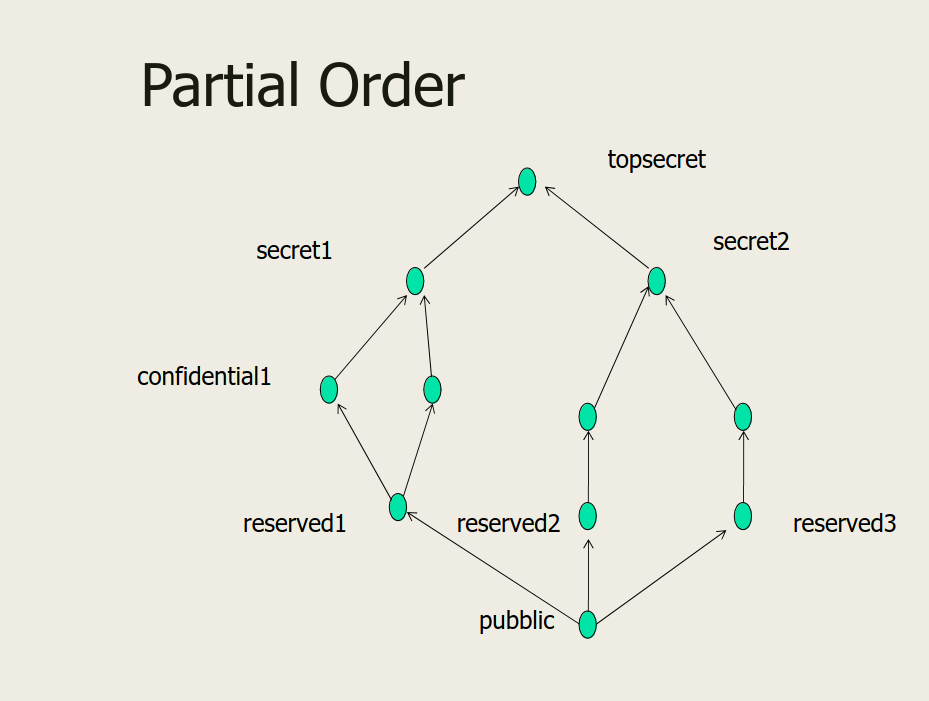
\includegraphics[width=0.5\textwidth]{images/partial_ordering.png}
\end{center}

% \section*{22 - Settembre}
Below are listed possible MAC (Mandatory Access Control) policies.
\paragraph{Bell-LaPadula}
Any subject $S$ in class $C$ is \textbf{allowed} to:
\begin{itemize}
    \item Read any file in a class $D \leq C$
    \item Write any file in $C$ class
    \item Append to any file in a class $D \geq C$
    \item Grant rights if $S$ is the owner and the previous contraints are satisfied
\end{itemize}
This a \textit{no write-down} policy, 
which preserves confidentiality and prevents an information flow from a higher to a lower level,
but may lead to information clustering in higher levels

\paragraph{Biba}
\begin{itemize}
    \item Read any file in $D \geq C$
    \item Write any file in $D \leq C$
\end{itemize}

Also called \textit{no write-up} policy, guarantees integrity but sacrificing condidentiality.

\paragraph{Watermark}
\textit{Time-dependant}, The level of a subject has maximum but is not fixed, it is the
highest one of the objects it has worked on, and increases anytime the
subject reads critical information.

\paragraph{No interference property}
Each object and each subject is paired with a label that
defines the corresponding level.
An object label is updated at run time according to both
\begin{itemize}
    \item the operations that are invoked
    \item the level of the subject invoking the operations
\end{itemize}

\paragraph{Clark-Wilson}
A policy in this class defines a set of \textbf{consistency constraints} on given objects and \textbf{sequences of operations} on the objects (\textit{well-formed transactions}) that preserve consistency constraints.

By allowing only such sequences, the system evolution can only navigate across states that satisfie the consistency constraints.

\paragraph{Chinese Wall}
As soon as $S$ invokes and operation on $Obj \in C$,
then:
\begin{itemize}
    \item $S$ cannot invoke operations on Objects $ \notin C$
    \item $S$ can invoke operations on Objects $ \in C$
\end{itemize}

\subsection{Overall Policy}
In a real world context, organizations merge several of the above-mentioned policies.
For a subject, the may be two distinct levels, one for \textit{confidentiality} and one for \textit{integrity}

\section{Trusted Computing Base}
TCB includes any modules involved in the implementation of the security policy.
TCB modules are critical, because any bug in one of these represents a vulnerability.\\
It is important to note that the security level (and the trust in it) is \textit{inversely proportional} to the \textbf{size} of the TCB,
since more lines of code imply higher chance to hide bugs,
hence vulnerabilities.

\section{Representing Security Policy}
It is possible to build an Access Control Matrix, where \lstinline|ACM[i,j]| indicates which operations subject \lstinline{I} can invoke on object \lstinline{j}.\\
Some kind of representation of ACM is a \textbf{necessary} and \textbf{not sufficient} condition to consider a policy valid and system actually secure. 
\begin{table}[h]
    \centering
    $S$
    \begin{tabular}{|c|c|c|}
        \multicolumn{3}{c}{$O$}\\
        \hline
         & &\\
         \hline
         & \textit{Rights} &\\
         \hline
         & & \\
         \hline
    \end{tabular}
    \caption{Access Control Matrix}
    \label{tab:ACM}
\end{table}